\documentclass[10pt,a4paper]{article}

\usepackage{amsmath}

\usepackage{inputenc}
\usepackage{fvextra}

\usepackage{algpseudocode}
\usepackage{algorithmicx}
\usepackage{amsfonts}
\usepackage{amssymb}
\usepackage{amsthm}
\usepackage[spanish]{babel}
\usepackage{bm}
\usepackage{booktabs} % To thicken table lines
\usepackage{bussproofs}
\usepackage{caption}
\usepackage{csquotes}
\usepackage{colortbl}
\usepackage{dsfont}
\usepackage{environ}
\usepackage[shortlabels]{enumitem}
\usepackage{fancyhdr}
\usepackage{forest}
\usepackage{geometry}
\usepackage{graphicx}
\usepackage[hidelinks]{hyperref}
\usepackage{ifthen}
\usepackage{multicol}
\usepackage{multirow}
\usepackage{sidecap}
\usepackage{stmaryrd}
\usepackage{tabularx}
\usepackage{titling}
\usepackage{tikz}
\usepackage{xcolor}
\usepackage{wrapfig}
\usepackage{minted}

\usetikzlibrary{arrows}
\usetikzlibrary{arrows.meta}
\usetikzlibrary{automata}
\usetikzlibrary{calc}
\usetikzlibrary{fit}
\usetikzlibrary{matrix}
\usetikzlibrary{positioning}
\usetikzlibrary{shapes.geometric}
\usetikzlibrary{shapes.multipart}

\newcommand{\red}[1]{{\color{red}#1}}
\newcommand{\green}[1]{{\color{green}#1}}
\newcommand{\blue}[1]{{\color{blue}#1}}
\newcommand{\violet}[1]{{\color{violet}#1}}
\newcommand{\orange}[1]{{\color{orange}#1}}

\newcommand{\nat}{\mathbb{N}}
\newcommand{\reales}{\mathbb{R}}

\newtheorem{theorem}{Teorema}
\newtheorem{coro}{Corolario}
\newtheorem{proposicion}{Proposición}
\newtheorem{lema}{Lema}


\usetikzlibrary{shapes.multipart}

\tikzstyle{demoBox} = [
draw=blue!20, very thick,
rectangle split, rectangle split parts=2, rounded corners, inner xsep=0.5cm,
rectangle split part fill = {blue!20, blue!5}
]

\tikzstyle{demoPart} = [
draw=blue!20, very thick,
rounded corners, inner xsep=0.5cm,
fill = blue!5
]
%\newcommand{\qed}{\begin{flushright}
%		$\blacksquare$
%\end{flushright}}

\NewEnviron{demo}[1][]{%
	\begin{center}
		\begin{tikzpicture}
			\node [demoBox](box){%
				\textbf{\scriptsize
					DEMOSTRACIÓN #1}
				\nodepart{two}
				\begin{minipage}{0.75\textwidth}
					\vspace*{0.1cm}
					\BODY
				\end{minipage}
			};
		\end{tikzpicture}
	\end{center}
}

\NewEnviron{demoPart}[1][]{%
	\begin{center}
		\begin{tikzpicture}
			\node [demoPart](box){%
				\begin{minipage}{0.75\textwidth}
					\vspace*{0.1cm}
					\BODY
				\end{minipage}
			};
		\end{tikzpicture}
	\end{center}
}


\title{Sistemas Operativos - Apuntes para final}
\author{Gianfranco Zamboni}

\usemintedstyle[cpp]{bordeland, tabsize=2}
%%%% CONFIGURACIONES %%%%

%% La coma de los reales es un punto
\decimalpoint{}

%%% Tamaño de pagina
%\geometry{
%	includeheadfoot,
%	left=2.54cm,
%	bottom=1cm,
%	top=1cm,
%	right=2.54cm
%}

%\stul{0.1cm}{0.2ex}

%% HEADER Y FOOTER
\pagestyle{fancy}

\fancyhf{}

\fancyhead[LO]{\rightmark} % \thesection\ 
\fancyhead[RO]{\small{\thetitle}}
\fancyfoot[CO]{\thepage}
\renewcommand{\headrulewidth}{0.5pt}
\renewcommand{\footrulewidth}{0.5pt}
\setlength{\headsep}{1cm}
\setlength{\headheight}{13.07225pt}

\renewcommand{\baselinestretch}{1.2}  % line spacing

%% Links en indice 
\hypersetup{
	linktoc=all,     %set to all if you want both sections and subsections linked
	linkcolor=blue,  %choose some color if you want links to stand out
}
\setcounter{tocdepth}{2}
\begin{document}

	\maketitle
	\tableofcontents

\newpage
\section{Introducción a la teoría de la información}
\subsection{La semilla del internet }

El telégrafo fue el antecesor del teléfono, un primer acercamiento a la comunicación de
mensajes vía una codificación. Desde fines de siglo XIX hasta segunda mitad del siglo XX,
aparecen las centrales de \textbf{conmutación de circuitos} (centrales telefónicas). A estas centrales
llegaban señales (cables) correspondientes a todas las casas que participacen en el sistema de
teléfonos. Las operadoras conectaban dos circuitos en sus tableros para cerrar el circuito y
permitir la comunicación entre las dos partes involucradas. Sin embargo, este tipo de comunicación tenía una gran falla: Si una central de conmutación de circuitos
dejaba de estar disponible por algún motivo de fuerza, todas las personas pertenecientes a esa
zona se verían incomunicadas.


A fines de los 50 se empieza a desarrollar la \textbf{conmutación de paquetes} buscando resolver este tema, es decir se busca una \textbf{red más tolerante a fallas}, \textbf{más flexible} a la hora de conectar dos puntos distantes y que \textbf{escale más facilmente} ante un incremento en el acceso a la comunicación.

La nueva red propuesta es una red descentralizada con mútiples caminos entre dos puntos que divide los paquetes en fragmentos que pueden llegar a destino a través de distintos caminos.

\subsection*{El modelo OSI}
En 1983 aparece una publicación de ISO para establecer un estándar que especifique la estructura de una arquitectura de red, que uniformice la forma de construir las redes de cominucación: el modelo OSI-ISO (Open Systems Interconnection).

\begin{figure}[h]
	\centering
	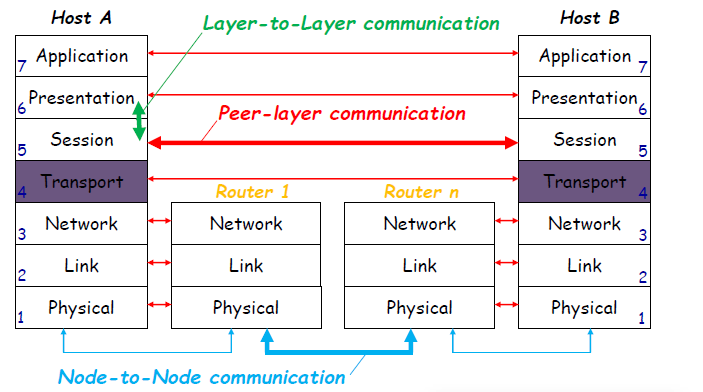
\includegraphics[width=0.65\textwidth
]{images/osi.png}
	\caption[Modelo OSI de Referencia]{Modelo OSI}
	\label{fig:osi}
\end{figure}

Este modelo está dividido en 7 capas, cada una de las cuales tiene una función definida que permitirán la comunicación coherente entre dos sistemas remotos.  

\begin{enumerate}
  \item La capa \textbf{física (Physical)} se encarga de enviar raw bits a través de los medios físicos disponibles en la red. 
  \item La capa de \textbf{enlace (Link)} se encarga de detectar errores en la transmisión y corregirlos, si es posible.
  \item La capa de \textbf{red (Network)} se encarga de resolver problemas de congestión dentro de la red, que paquetes se aceptan y la ruta que deben tomar los paquetes que se envían por la misma.
  \item La capa de \textbf{transporte (Transport)} se encarga de tomar la información provista por la capa de arriba, pasarla a la capa de red separada en pedazos más chicos (\textbf{chunks}) y se asegura que todas las partes lleguen a destino correctamente. 
  
  Esta es la primer capa \textbf{end-to-end}, es decir que entabla una "conversación" entre la máquina emisora (\textbf{Source}) y la destinataria (\textbf{Destination}). Las capas anteriores, usan protocolos de comunicación nodo a nodo, es decir, entre una máquina y su vecino inmediato y no entre el source y el destination que podrían estar separados entre sí por varios nodos.
  
  \item La capa de \textbf{sesión  (Session)} permite establecer sesiones entre dos máquinas distintas. Estas sesiones permiten sincronizar el pasaje de información entre ambas máquinas, deciden de quien es el turno para enviar información y evitar que ambas máquinas realizen operaciones críticas de manera simultanea.
  \item La capa de \textbf{presentación (Presentation)} procesa la información recibida, la estructura y la codifica de la manera necesaria para que pueda ser usada por la máquina.
  \item La capa de \textbf{aplicaciones (Application)} contiene los protocolos necesarios para que los usuarios puedan ver y leer la información.
\end{enumerate}

Además de estas funcionalidades, cada capa ofrece una interfaz que le permite comunicarse con las capas vecinas para hacer el pasaje de los datos entre ellas y asumen que el host en el otro extremo de la comunicación tendrá una arquitectura similar y podrá interpretar los mensajes de cada una de ellas.

\subsection{Modelo TCP/IP}
\begin{figure}[H]
	\centering
	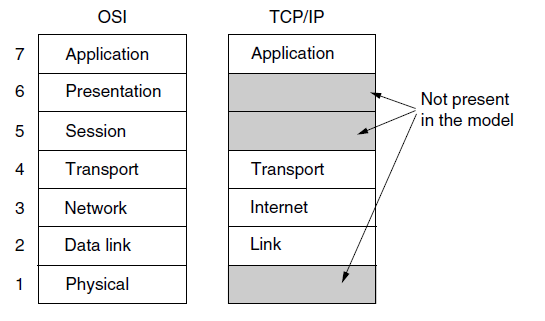
\includegraphics[width=0.65\textwidth
]{images/tcpip.png}
	\caption[Modelo TCP/IP de Referencia]{Modelo TCP/IP}
	\label{fig:tcp}
\end{figure}
Fue diseñado con el objetivo de mantener las conexiones intactas mientras ambos puntos finales de conexión estén funcionando, incluso si laguno de las máquinas o líneas entre ellos fuese dado de baja.

\begin{enumerate}
  \item La capa de \textbf{enlace (Link)} describe que deben cumplir los enlaces (cable de ethernet, lineas telefónicas, etc) para poder usados como medios de trasporte para este tipo de conexión.
  \item La capa de \textbf{intrared (internet)} permite al host injectar paquetes en cualquier red y se encarga de hacerlos llegar a destino. Esto se hacer de manera independiente para cada paquete, es decir pueden no seguir el mismo camino e incluso podrían llegar en distinto orden. En el último caso corresponde a la capas superiores reodenarlos para que puedan ser procesados, si es necesario.
  \item La capa de \textbf{transporte (Transport)} debe ser diseñada para permitir que dos entidades de la red puedan mantener una conversación. Aquí se definieron dos protocolos:
  \begin{itemize}
    \item El \textbf{Transmission Control Protocol (TCP)} que permite enviar sin errores un stream de bytes desde una máquina a otra en la red.
    \item El \textbf{User Datagram Protocol (UDP)} que permite evitar todo el flujo de conexión TCP y crear el suyo propio. En general, se usa en aplicaciones que requieren una respuesta más rápida que precisa. 
  \end{itemize}
  \item La capa de \textbf{Aplicación (Application)} que se incluye la sesiones y funciones necesarias para codificar y procesar los paquetes enviados y recibidos. Entre los protocolos usados en esta capa se encuentran: TELNEt, FTP y SMTP.
\end{enumerate}

\newpage
\section{Nivel físico}
\begin{figure}[H]
	\centering
	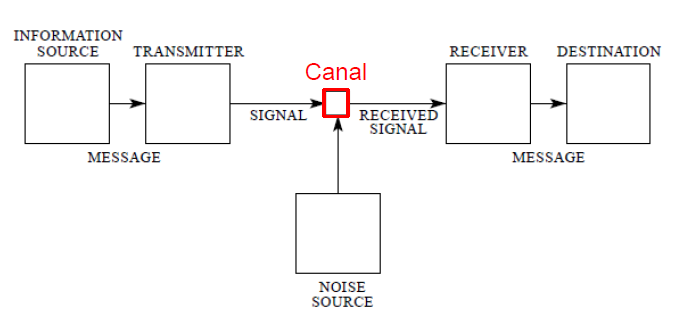
\includegraphics[width=0.65\textwidth
]{images/sistema-comunicacion.png}
	\caption[Esquema general de un sistema de comunicación]{Esquema general de un sistema de comunicación}
	\label{fig:sistema-comunicacion}
\end{figure}
Cuando enviamos un mensaje a una máquina en una red, debemos pasar ese mensajes por un \textbf{transmisor} que convertirá el mensaje en una serie de \textbf{señales} que pueden ser enviadas a través del \textbf{canal} que nos comunica con la máquina de \textbf{destino}. La máquina de destino debe tener un \textbf{recibidor} que le permita captar las señales del canal y transformarlas nuevamente en el mensaje original.


Sin embargo, los canales de transmisión físicos no son perfectos y aportan \textbf{ruido} a las señales emitidas por nuestro transmisor pudiendo llegar a destino con errores.

\begin{figure}[H]
	\centering
	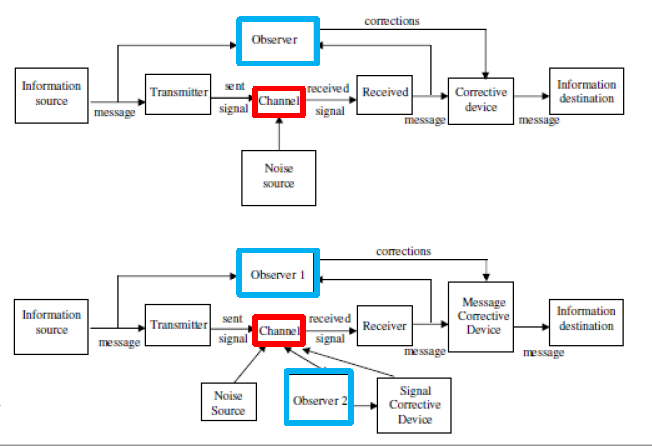
\includegraphics[width=0.65\textwidth
]{images/sistema-comunicacion-correccion.png}
	\caption[Esquema general de un sistema de comunicación]{Esquema general de un sistema de comunicación}
	\label{fig:sistema-comunicacion-correccion}
\end{figure}
Una forma de tratar de resolver esto es agregar, al modelo, nuevas capas de actores que trabajan para reducir los efectos nocivos del ruido. Por ejemplo, podemos agregar al modelo observadores externos que sean capaces de ver lo que se transmite de un lado y se recibe del otro, deducir información a partir de las diferencias, y tener chance de enviarle
correcciones al Elemento Corrector. También es posible tener dos niveles de observadores:
uno que se maneja a nivel mensaje y otro que se maneja a nivel característica del canal
propio.
\subsection{Fundamentos de las señales}
Las señales que se envían por el canal físico para comunicar dos extremos de un canal son \textbf{ondas electromagnéticas} que se propagan a través del canal a una cierta velocidad determinada por el tipo de canal que estemos usando.

Esta onda se desplaza longitudinalmente sobre un plano \textbf{vibrando} a auna \textbf{frecuencia} \(f\) determinada con un comportamiento periódico en el eje de su propagación.

En base a este período definimos su \textbf{longitud de onda} \(\lambda\) como:
\[\lambda = \frac{c}{f}\] donde \(c=3*10^8\frac{m}{s}\) es la velocidad de la luz.

Esta onda puede chocar con imperfecciones del material (del canal), producir reflexiones y refracciones que se tranducen en \textbf{perdidas} (menos energía para la señal original en la que está codificado el mensaje)

Dado que las ondas electromagnéticas son continuas y que son modificadas a medida que se propagan por el canal, debemos encontrar una manera de mapear estas frecuencias a los 0 y 1 que componen nuestros mensajes.

Para esto, tanto el transmisor como el recibidor definen un \textbf{ancho de banda} que es el rango de frecuencias que va a ocupar las señales que van a ser transmitidas por el canal y dentro de ese rango, cuales deben ser mapeadas a un 1 y cuales a un 0.

\subsection{Teoría de la información}
\subsubsection{Información}
Sea \(E\) un suceso que puede presentarse con probabilidad \(P(E)\). Cuando \(E\) tiene lugar, decimos que hemos recibido \[I(E)=\log\frac
{1}{P(E)}\] unidades de información.

Si introducimos el logaritmo de base 2, la unidad se denomina \textit{bit}. Notemos, también, que si \(P(E) = \frac{1}{2}\), \(I(E) = 1\) bit. Es decir, un bit es la cantidad de información obtenida al especificar una de dos posbiles alternativas igualmente probables.

\subsubsection{Fuentes de Memoria Nula}
Son fuentes de información que emiten una secuencia de símbolos pertenecientes a un alfabeto finito y fijo \(S=\{s_1,\dots,s_n\}\) de manera estadísticamente independientes. Estas fuentes pueden describirse mediante el alfabeto \(S\) y las probabilidades con que los simbolos se presentan: \(P(s_1), \dots, P(s_n)\).

La información que aporta cada símbolo de la fuente \[I(s_i) = \log_2\frac{1}{P(s_i)}\text{ bits}\]
\subsubsection{Entropía}
Dada una fuente de memoria nula \(S\) con alfabeto \({s_1,\dots,s_n}\), la entropía \(H(S)\) es la cantidad media de información por símbolo de la fuente, es decir:
\[H(S) = \sum_{i=1}^n P(s_i)I(s_i) = \sum_{i=1}^n P(s_i)\log_2\frac{1}{P(s_i)} = -\sum_{i=1}^n P(s_i)\log_2 P(s_i)\text{ bits} \]

Podemos interpretar la entropía como el \textbf{valor medio ponderado de la cantidad de información} del conjunto de mensajes posibles, como una medida de la \textbf{incertidumbre probmedio (grado de incerteza)}acerca de una variable aleatoria o la \textbf{cantidad de información} obtenida al observar la aparición de cada nuevo símbolo.

\paragraph{Propiedades:}
\begin{itemize}
  \item La entropía es no negativa y se anula si y solo si la probabilidad de uno de sus símbolos es 1 y la del resto es 0.
  \item La entropía máxima (\textbf{mayor incertidubme del mensaje}) se logra cuando todos los símbolos que puede ser emitidos por la fuente son equiprobables.
  \item Si hay \(n\) símbolos equiprobables \(P(s)=\frac{1}{n}\) se cumple:
    \[
      H(S) = -\sum_s P(S)\log_2 P(S) = -n(\frac{1}{n}\log_2\frac{1}{n}) = -(\log_2 1 - log_2 n) = \log_2 n
    \]
\end{itemize}

\subsubsection{Codificación}
Dado un alfabeto fuente \(\Sigma\), un código es una correspondencia entre todas las secuencias posibles de símbolos de \(\Sigma\) a secuencidas de símbolos de un alfabeto código \(X\).

Cuando codificamos un alfabeto fuente, buscamos logra una representación eficiente de la información mediante la eliminación de la redundancia.

Un código es \(C:\Sigma\to X^*\):
\begin{itemize}
  \item \textbf{Bloque:} Si asigna a cada símbolo una secuencia fija  de símbolos de \(X\).
  \item \textbf{No singular:} Si todas sus palabras son distintas. Es decir si \(C\) es una función inyectiva.
  \item \textbf{Separable o Univócamente Decodificable:} Si ninguna tira de símbolos del alfabeto código admite más de una única decodificación.
  \item \textbf{Instantáneo:} Si cumple la condición libre de prefijos: No existe ninguna palabra que sea prefijo de otra palabra de longitud mayor. Si tenemos este tipo de código entonces cuando el receptor recibe una palabra sabé como tiene que decodificarla, sin la necesidad de esperar más bits.
  
  Si un código es instantaneo entonces en univócamente decodificable. 
\end{itemize}

\paragraph{Inecuación de Kraft:} Dado un alfabeto \(S = \{s_1,\dots,s_n\}\) y un alfabeto de código \(X=\{x_1,\dots,x_m\}\), es condición necesaria y suficiente, para exista un código instantáneo con palabras de longitud \(l_1,\dots,l_{n}\), que se cumpla la siguiente inecuación:
\[\sum_{i=1}^n |X|^{-l_1}\leq 1\]
\paragraph{Codificación eficiente:} Buscamos codificar un alfabeto \(S\) de tal forma que máximizar la relación entre la entropía \(H(S)\) y la longitud media del código \(L\):  Sea \(L_i\) la longitud de la palabra que codifica al símbolo \(s_i\) de la fuente, \(p_i\) la probabilidad de aparicion de \(s_i\) y \(r\) la cantidad de símbolos diferentes en el alfabeto del código entonces:

\begin{itemize}
  \item \(L = \sum p_iL_i \) es la longitud medía del código.
  \item \(\log r\) es la cantidad promedio máxima de información de un símbolo del código.
  \item \(h = \frac{H(S)}{L\log r}\) es la eficencia del código.
\end{itemize}

La máxima eficencia se logra cuando \(h = 1\). En general, esto sucede cuando se asigna las palabras de código más cortas a los símbolos de fuente más probables.

\paragraph{Codificador óptimo:} Es un codificador que usa la menor cantidad posible de bits para codificar un mensaje, es decir: Un codificador se dice óptimo si no existe ningún código para la misma fuente con menor longitud media.

Sea \(s_i\in S\), entonces la cantidad de bits necestarios para representarlo en un codificador óptimo es \(\lceil\frac{1}{P(s)}\) y la entropía de \[H(X) = \sum_{s\in S} P(s)\log_2\left(\frac{1}{P(s)}\right)\]

\paragraph{Codificación de Huffman:} Este método obtiene codificadores óptimos armando un árbol de prioridades en base a la frecuencia de aparición de cada símbolo en un mensaje.

\subsection{Los medios de transmición reales}
Estos son los pasos necesarios a realizar durante el envio de datos a través de un canal:
\begin{enumerate}
  \item Una fuente emite un mensaje hacia un codificador que lo transforma en una secuencia de bits a partir de una codificación idealmente eficiente.
  \item El mensaje codificado en bits, pasa a un codificador de canal que se encarga de transformar esos bits a frecuencias para que puedan ser trasmitidos. Muchas veces, se agrega redundancia para ayudar a combatir el ruido del canal.
  \item Del otro lado del canal, sucede el proceso inverso: Un decodificador de canal lee las frecuencias y las trasnforma a una secuencia de bits para que, luego, el decodificador del mensaje, la transforme en el mensaje original enviado por la fuente.
\end{enumerate}

\begin{figure}[H]
	\centering
	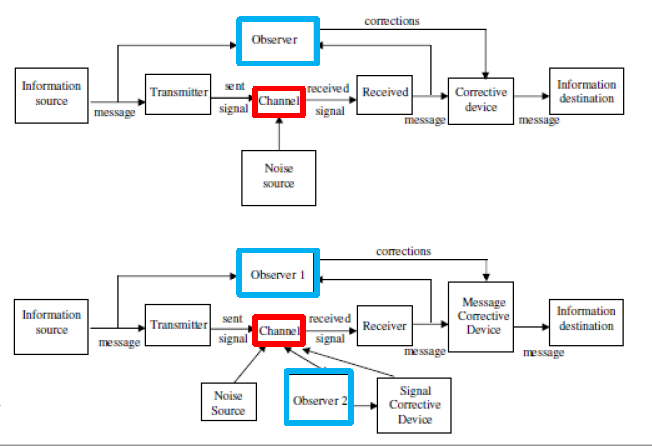
\includegraphics[width=0.65\textwidth
]{images/sistema-comunicacion-correccion.png}
	\caption[Esquema general de un sistema de comunicación]{Esquema general de un sistema de comunicación}
	\label{fig:sistema-comunicacion-real}
\end{figure}
\subsubsection{Problemas de los canales físicos}
Como los canales de transmición existentes no son perfectos, la señal recibida por el decodificador puede diferir de la transmitida debido a una gran variedad de tipos de errores:

\begin{itemize}
  \item \textbf{Atenuación:}  En medios análogicos, la señales se degradan con la distancia recorrida lo que puede llevar a provocar errores en algunos bits recibidos. Por lo que la intensidad de la señal recibida deber ser suficiente para ser detectada y, además, debe ser suficientemente mayor al ruido del canal para que se reciba sin error. En general, las frecuencias más afectadas son las más altas por lo que se puede ecualizar estas frecuencias, es decir, amplificarlas.
  \item \textbf{Distorsión de retardo:} En medios guiados, la velocidad de propagación en el medio varía con la frecuencia por lo que los componentes del mensaje llegan en distintos instantes de tiempo, originando desplazamiento de fases entre las distintas frecuencias.
\item \textbf{Ruido:} Los canales físicos poseen ruido natural. Es decir, transmiten señales adiciones debido a agentes externos:
\begin{itemize}
  \item \textbf{Ruido Término ó Ruido Blanco:} Se produce debido a la agitación térmica de electrones y aumenta linealmente con la temperatura absoluta del canal.
  \item\textbf{Ruido por intermodulación:} Son señales que son la suma o la diferencia de sus frecuencias originales producidas por una falta de linealidad en el canal.
  \item\textbf{Ruido por Diafonía:} Se produce cuando una señal de una línea interfiere en otra.
  \item\textbf{Ruido impulsivo:} Son impulsos irregulares o picos que se pueden producir por interferencias externas (como pueden ser interferencia electromagnéticas, tormentas, etc). Este tipo de ruido es de corta duración, tienen gran amplitud y es disruptivo.
\end{itemize}
\end{itemize}

\subsubsection{Capacidad de un canal}
Estas perturbaciones afectan la velocidad de transmición del canal por lo que debemos asegurarnos de no enviar más bits que la capacidad límite del mismo para no perder información durante la transmición. Para esto vamos a definir los siguientes conceptos:

\begin{itemize}
  \item Vamos a nombrar \(C\) a la capacidad del canal, es decir a la cantidad de bits por segundo que podemos transmitir a través del mismo.
  \item \(B\) es el ancho de banda por el cual vamos a transmitir nuestros datos, va estar medido en ciclos por segundo (Hertz) y va estar limitado por el transmiso y el medio.
  \item \(N\) es el nivel medio o potencia del ruido del canal
  \item \(BER\) es la tasa de errores de bits por segundo (Bit Error Rate).
  \item \(S\) es la potencia o amplitud de la señal.
  \item \(SNR = S / N\) es la relación señal a ruido medido en decibeles.
\end{itemize}

\[C = B\log_2(1 + SNR)\]

En principio, si se aumentan el ancho de banda \(B\) y la potencia de señal \(S\), aumenta la velocidad binaria. Sin embargo, un aumento de \(B\) aumenta el ruido y un aumento de \(S\) aumenta las no linealidades y el ruido de intermodulación.

\begin{figure}[H]
	\centering
	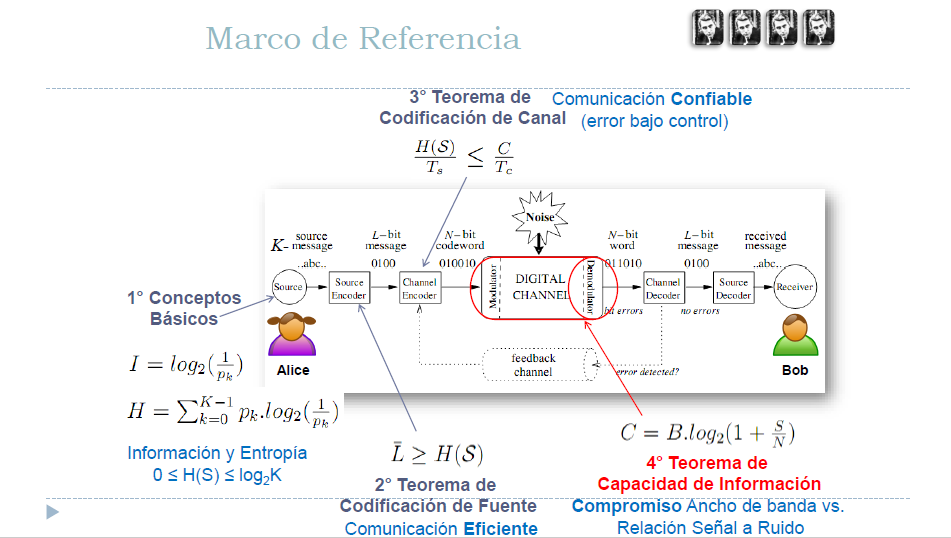
\includegraphics[width=\textwidth
]{images/marco-referencia.png}
	\caption[Esquema de un sistema de comunicación y sus conceptos asociados]{Esquema de un sistema de comunicación y sus conceptos asociados}
	\label{fig:marco-referencai}
\end{figure}


\paragraph{Límite de eficencia:} La eficiencia de ancho de banda es la máxima cantidad de bits por segundo que podemos inyectar por cada Hz sin perder información. Mientra más eficiente sea el canal, se pueden transmitir más bits por segundo. 

\paragraph{Límie de confiabilidad:} \red{Es la cantidad máxima de bits por segundos que podemos utilizar para transportar una señal de manera confiable a través de un canal ruidoso}
\red{
Ancho de banda. Medios de transmisión guiados y no guiados. Punto a Punto y Compartidos (Broadcast). Modems. Modulación: Fase, Frecuencia, Amplitud y QAM. Conversión Analógico/Digital. Capacidad de Canal. Latencia. Producto delay-ancho de banda.

\section{Nivel Enlace}
Punto a Punto. Servicios. Entramado. Manejo del enlace. Control de flujo. Control de errores: detección y corrección. Distancia de Hamming. Protocolo Stop \& Wait. Protocolos de ventana deslizante. Comparación de protocolos. Medidas de eficiencia.

\section{Medios Compartidos}
Compartidos. Redes locales (LANs). Generalidades. Medios de transmisión. Nivel físico. Nivel de enlace de datos. Subcapa LLC (Logical Link Control): IEEE802.2. Subcapa MAC (Medium Access Control): IEEE 802.3 (Ethernet). CSMA/CD. Redes Inalámbricas. Frecuencia dedicada versus expandida (Spread Spectrum). WLANs. CSMA/CA. Wi-Fi: IEEE 802.11b/g/n. Repetidores. Puentes. LAN Switches. Conceptos de VLAN y troncales de VLANs (IEEE 802.1Q). Spanning Tree Protocol.

\section{Nivel Red}
Conmutación y Forwarding. Subredes. Implementación: circuitos virtuales y datagramas. Control de flujo. Concepto de Ruteo. Protocolo IP. Direccionamiento. Broadcasting. Ejemplos de subnetting. Protocolo ARP. Forwarding. ICMP. Traducción de direcciones (NAT).

\section{Ruteo Externo e Interno}
Distance Vector y Link State. Los protocolos RIP y OSPF. Áreas. Inundación confiable.

\section{Nivel de transporte}
Servicios. Primitivas. Protocolos. Servidores de nombres. Manejo de conexión: establecimiento, uso y liberación. Manejo de conexión basados en tiempo. Direccionamiento. Control de flujo. Asignación de buffers. Recuperación de caídas. Multiplexado. Protocolos de nivel 4: Transport Control Protocol (TCP). User Datagram Protocol (UDP) . Mecanismos de control de congestión. Cálculo del RTO. Control de Flujo. Control de errores. Determinación de la performance.

\section*{Congestión}
Introducción al problema de congestión. Curvas de Trafico Enviado vs entregado. Resultado con buffer infinito. Causas de congestión. Control de flujo vs Control de congestión. Taxonomia de Yang y Redan. Soluciones de lazo cerrado y abierto. Concepto de sistemas realimentados. Métricas a sensar para las realimentación. Realimentación implícita y explicita. Determinación de la performance.

\section{Aplicaciones}
Aplicaciones. Correo Electrónico. Protocolos : SMTP, POP3 e IMAP, MIME. Servidores World Wide Web. HTTP. Servidor de Nombres: DNS. Jerarquía de dominios. Resolución de nombres.

\section{Seguridad}
Seguridad en Redes. Marco de Trabajo. Criptografía. Seguridad. Privacidad. Protocolos de Clave Pública y Privada. Algoritmos: DES, 3DES, AES, RSA, MD5 y SHA .Ventajas y desventajas de cada uno. Sus aplicaciones (Autorización, Firma, Confidencialidad e Integridad). Distribución de Claves Públicas. Firewalls. Tunneling. Conceptos de amenazas, ataques, intrusiones.
}
\end{document}

